\documentclass[tikz,border=2mm]{standalone}
\definecolor{structure}{HTML}{1A535C}
\definecolor{main}{HTML}{C6892A}
\definecolor{third}{HTML}{8B2635}

\begin{document}

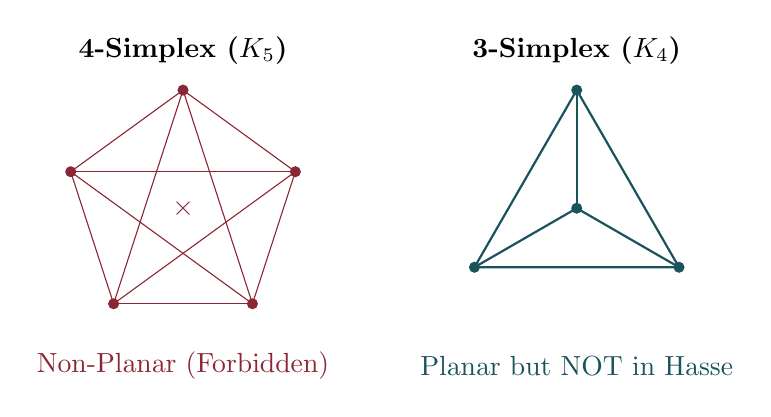
\begin{tikzpicture}[scale=1]

% Left: K5 (Non-Planar)
\begin{scope}[shift={(-2.5,0)}]
    \node at (0, 2) {\textbf{4-Simplex ($K_5$)}};
    \node at (0, -2) {\color{third} Non-Planar (Forbidden)};
    
    % Pentagon vertices
    \foreach \i in {1,...,5} {
        \coordinate (v\i) at (90-\i*72:1.5);
        \fill[third] (v\i) circle (2pt);
    }
    % Edges (Complete Graph)
    \foreach \i in {1,...,4} {
        \foreach \j in {\i,...,5} {
            \draw[third, thin] (v\i) -- (v\j);
        }
    }
    % Highlight crossings
    \node[circle, fill=white, inner sep=1pt] at (0,0) {\color{third}$\times$};
\end{scope}

% Right: K4 (Planar but forbidden in Hasse)
\begin{scope}[shift={(2.5,0)}]
    \node at (0, 2) {\textbf{3-Simplex ($K_4$)}};
    \node at (0, -2) {\color{structure} Planar but NOT in Hasse};
    
    % Triangle vertices
    \coordinate (a) at (90:1.5);
    \coordinate (b) at (210:1.5);
    \coordinate (c) at (330:1.5);
    \coordinate (center) at (0,0);
    
    \fill[structure] (a) circle (2pt);
    \fill[structure] (b) circle (2pt);
    \fill[structure] (c) circle (2pt);
    \fill[structure] (center) circle (2pt);
    
    % Edges
    \draw[structure, thick] (a) -- (b) -- (c) -- cycle;
    \draw[structure, thick] (center) -- (a);
    \draw[structure, thick] (center) -- (b);
    \draw[structure, thick] (center) -- (c);
    
    % No crossings!
\end{scope}

\end{tikzpicture}

\end{document}
